\section{DeepScope: A Deep Image of the City}\label{sec:deepscope}

{
    \subsection{Introduction}
    {
        As discussed in previous sections, predicting the impacts of city-planning can help evaluate the future performance of different urban systems - from mobility and energy to safety and economic development (see Sections \eqref{sec:cityscope_volpe}, \eqref{sec:grasbrook}, \eqref{sec:modeChoices}). Nevertheless, more subtle aspects of planning, such as the physical appearance of development, are not easily predicted or evaluated during early planning stages.
        \newline
        Urban-design renderings and streetscape visualizations are commonly used by designers, stakeholders, and decision-makers to asses future design. These visual aids can clarify the outcomes of design decisions, such as zoning, building codes or land-use allocations, and can affect urban development for decades to come \cite{al1999using, smith1998visual}. Yet despite major advancements in computer graphics, rendering, and visualization tools, crafting quality urban visualizations is still a complex, lengthy and costly task. This work introduces \textit{DeepScope}, a CityScope module for real-time urban-design visualizations. DeepScope utilizes a Generative Neural Network (DCGAN \cite{mirza2014conditional}) designed for real-time feedback. The rest of this section details the design and the implementation of DeepScope.

        \subsubsection{`Imageability'}
        {
            \emph{``To understand the role of environmental images in our own urban lives (...) we needed to develop and test the idea of imageability (...) and thus to suggest some principles for urban-design.''} \cite{lynch1960image}


            \begin{figure}[!htb]
                \centering
                \includegraphics[width=1\columnwidth]{chapters/prediction/deepscope/figures/deepscope5.png}
                \caption{Urban `Imageability'. (left) Kevin Lynch's imageability classification metric for street element and urban experience. (right) An example street view, in which many of these classes are homogeneously interconnected \cite{lynch1960image}.}~\label{fig:deepscope_lynch}
            \end{figure}

            In 1960, MIT professor and Urbanist Kevin Lynch, introduced the idea of urban `imageability': a novel approach to visual perception of the built environments \cite{lynch1960image}. Lynch suggested a new classification of city-form, in which nodes, landmarks, paths, edges and districts reflect the sensation of traversing through the urban scape. Figure \eqref{fig:deepscope_lynch} demonstrates Lynch's imageability  and their manifestation in the streetscape. In the 1964 `The View From the Road' study \cite{appleyard1964view}, Lynch tested the idea of `imageability' using a new medium: He mounted a film camera to a car dashboard, and went on several day rides around five US metros \cite{Andrews2007}. When later played, these recordings were sped to reflect the overall `feel' of the urban skyline, overlooking nuanced street elements and architectural details, and prompting questions such as: What is the composition of the built mass? What shapes the street-section? Are there any noticeable landmarks, forms, or gaps? \cite{carr1969city, pearce1996legacy}.
        }

        \subsubsection{Urban Visualization}
        {
            Lynch's work contributed to the notion that street-level views are critical during initial urban-design stages, when the urban context is only being established \cite{drettakis2007design, brusaporci2017importance}. In the last few decades, advancements in computer graphics made it easier to visualize future urban developments \cite{shiode20003d, kempenaar2016design}. Nevertheless, few tools provide realistic and real-time urban visualizations, which can also be used as part of collaborative design processes \cite{mueller2018citizen}.
            \newline
            Most common visualization tools carry complex setups, costly hardware and software, as well as steep learning curves \cite{yan2014evaluation, mekni2014augmented}. These tools often require users to set up many control parameters, such as cameras, lights, and materials, and constantly adjust these to produce decent results. This process can become laborious in complex design scenes, and can gravely affect the outcome, cost and duration of visualization processes, and the design process as a whole \cite{lovett2015using}.
        }
    }


    \begin{figure}[!htb]
        \centering
        \includegraphics[width=1\columnwidth]{chapters/prediction/deepscope/figures/deepscope3.png}
        \caption{From interaction to prediction. (left) TUI interactions are captured using OpenCV and streamed to the webGL app. A 3D model is created based on the grid's JSON array and the Observer viewing angle. Lastly, a snapshot image is fed as an input vector to the DCGAN model. (right) (1) Observer position (2) Observer view angle and FOV cone (3) Observer's 3D street-view as input for DCGAN (4) DCGAN model prediction of street-view (5) TUI interactive grid.}~\label{fig:deepscope_dataflow}
    \end{figure}



    \subsection{System Design}\label{DeepScope-system-architecture}
    {
        DeepScope is a CityScope module for collaborative, tangible, and real-time urban-design visualization. DeepScope allows multiple users to collaboratively observe the visual outcomes of early planning stages using autogenerated visualizations. As with other CityScope platforms, DeepScope requires minimal setup, basic hardware and software, and no expertise to use\footnote{For general design of CityScope platforms see Section \eqref{sec:cityscope_architecture}}.

        \subsubsection{DeepScope User Interaction}\label{DeepScope-user-interaction}
        {
            DeepScope TUI is composed of three components: (i) A physical urban model, (ii) a scanning module, and (iii) a feedback module. The urban model includes an arbitrary grid of LEGO tiles, tagged with binary patterns, and scanned using CityScoPy as discussed in Section \eqref{subsec:csarch-cityscopy}. Figure \eqref{fig:deepscope_users} depicts a user positioning a tagged LEGO brick into the TUI design space to trigger the model generation.

            \begin{figure}[!htb]
                \centering
                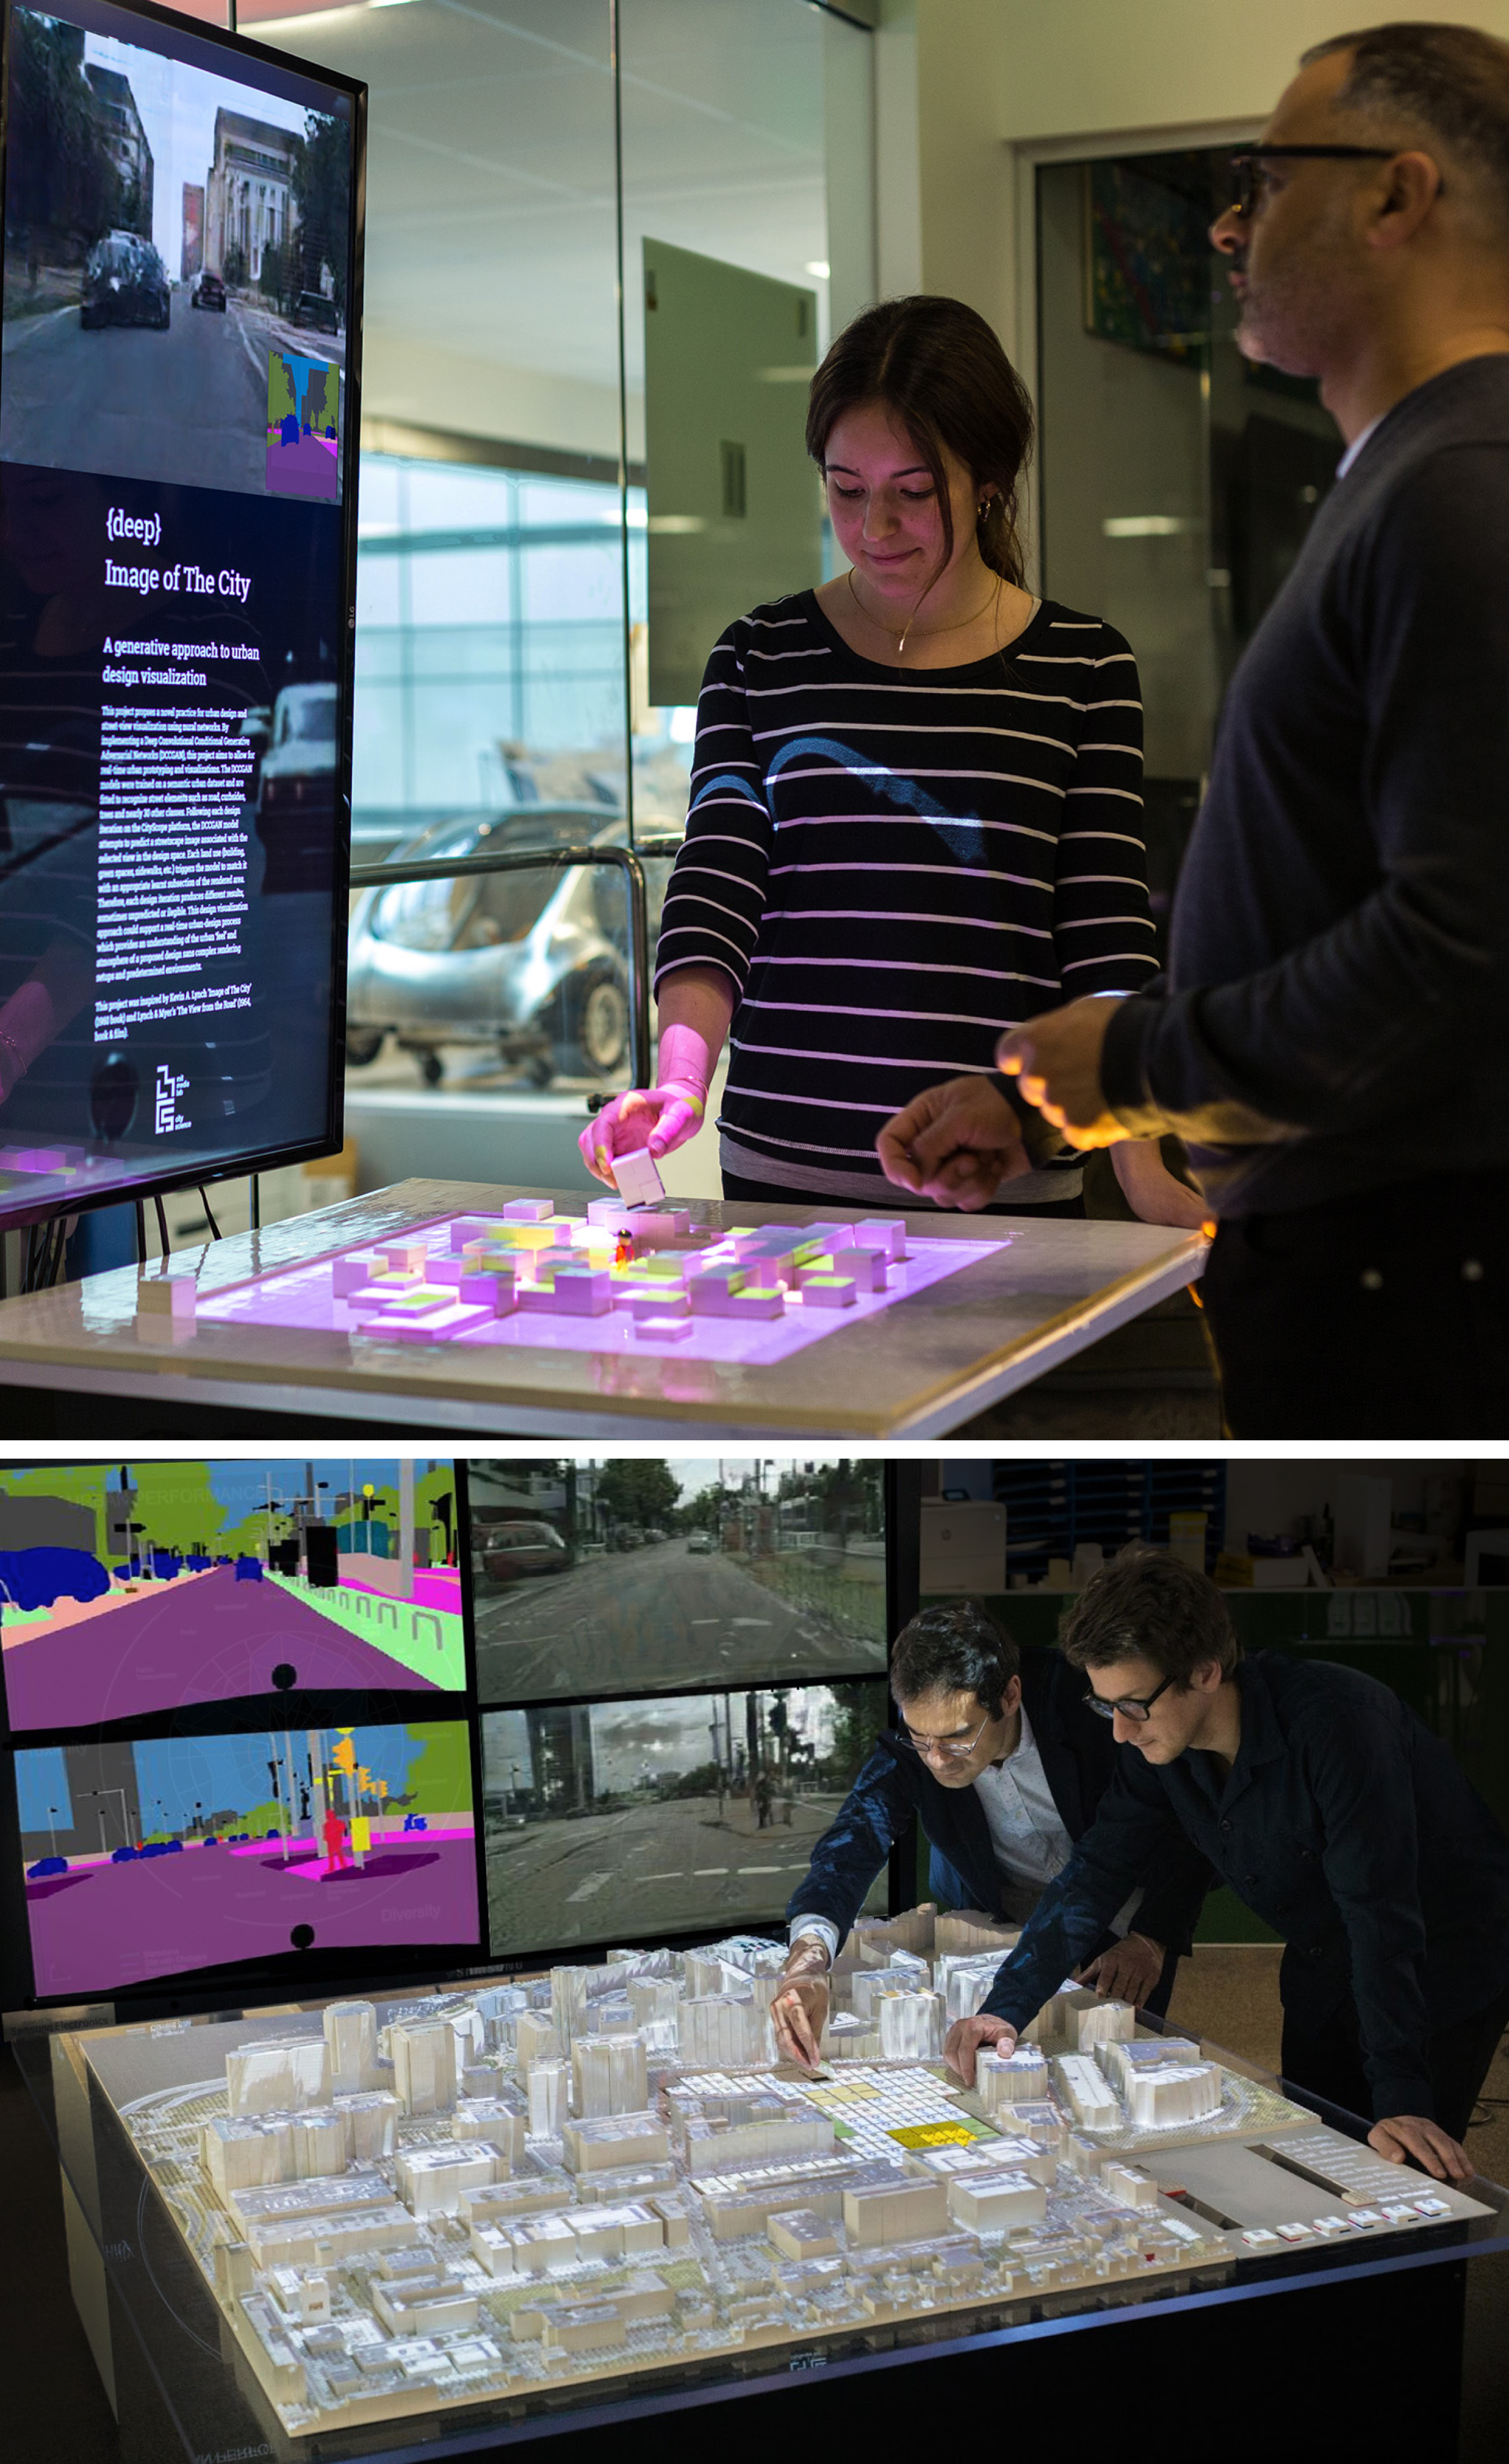
\includegraphics[width=0.6\columnwidth]{chapters/prediction/deepscope/figures/deepscope2.png}
                \caption{
                    Multi-user interaction with DeepScope.
                    Multiple users can simultaneously interact and discuss urban-design iterations. The table-top is used as both the design space and a schematic urban top-view. The vertical monitor visualizes the DCGAN street view.
                }~\label{fig:deepscope_users}
            \end{figure}

            In DeepScope, each grid-cell pattern represents a different streetscape class, such as roads, buildings, green-spaces, parking, or sidewalks. Each class contains additional parameters, such as height, volume, shape, rotation and density. Table \eqref{deepscope:tab-types-classes} specifies the classes and their attributes.


            \begin{table}
                \begin{center}
                    \caption{
                        Cityscapes dataset classes used in DeepScope. Marked with `plus' are labels which can be altered dynamically using CS TUI. Marked with `star' are labels that are generated dynamically in the 3D model.
                    }
                    \label{deepscope:tab-types-classes}
                    \begin{tabular}{l|l}
                        \hline
                        \textbf{Group} & \textbf{Classes}                                                     \\
                        \hline
                        flat           & road*+; sidewalk*+ parking*+; rail track                             \\
                        human          & person*; rider*                                                      \\
                        vehicle        & car*; truck*; bus*; on rails; motorcycle; bicycle*; caravan; trailer \\
                        construction   & building; wall*; fence; guard rail; bridge                           \\
                        object         & pole*; pole group; traffic sign*; traffic light*                     \\
                        nature         & vegetation*+; terrain                                                \\
                        sky            & sky*                                                                 \\
                        void           & ground; dynamic; static
                    \end{tabular}
                \end{center}
            \end{table}
        }

        \subsubsection{Procedural Environment}
        {
            With each user interaction, the scanner decodes the array of grid-cell patterns and updates the CityScope Schema (see Section \eqref{sec:cityscope_architecture}). This triggers a generation of a virtual 3D environment, in which each grid-cell is represented via its class and additional parameters (see Figure
            \eqref{fig:deepscope_dataflow}
            ). As users allocate tiles, the 3D environment is procedurally populated with streetscape elements. For example, a vegetation pattern will create a surface with procedural trees, bushes or live-fences; A sidewalk pattern will produce pedestrians and street-signage, and a parking-lot pattern will be proliferated with parked vehicles. The generated 3D environment is uniformly hued with RGB values that correspond to input classes which correspond to the Cityscape dataset classes, and are expected by the GAN model (see Section \eqref{DeepScope-Generative-Model}). The 3D scene generation is done on the client-side web-browser using WebGL and ThreeJS \cite{mrdoob_2019}.
        }


        \begin{figure}[!htb]
            \centering
            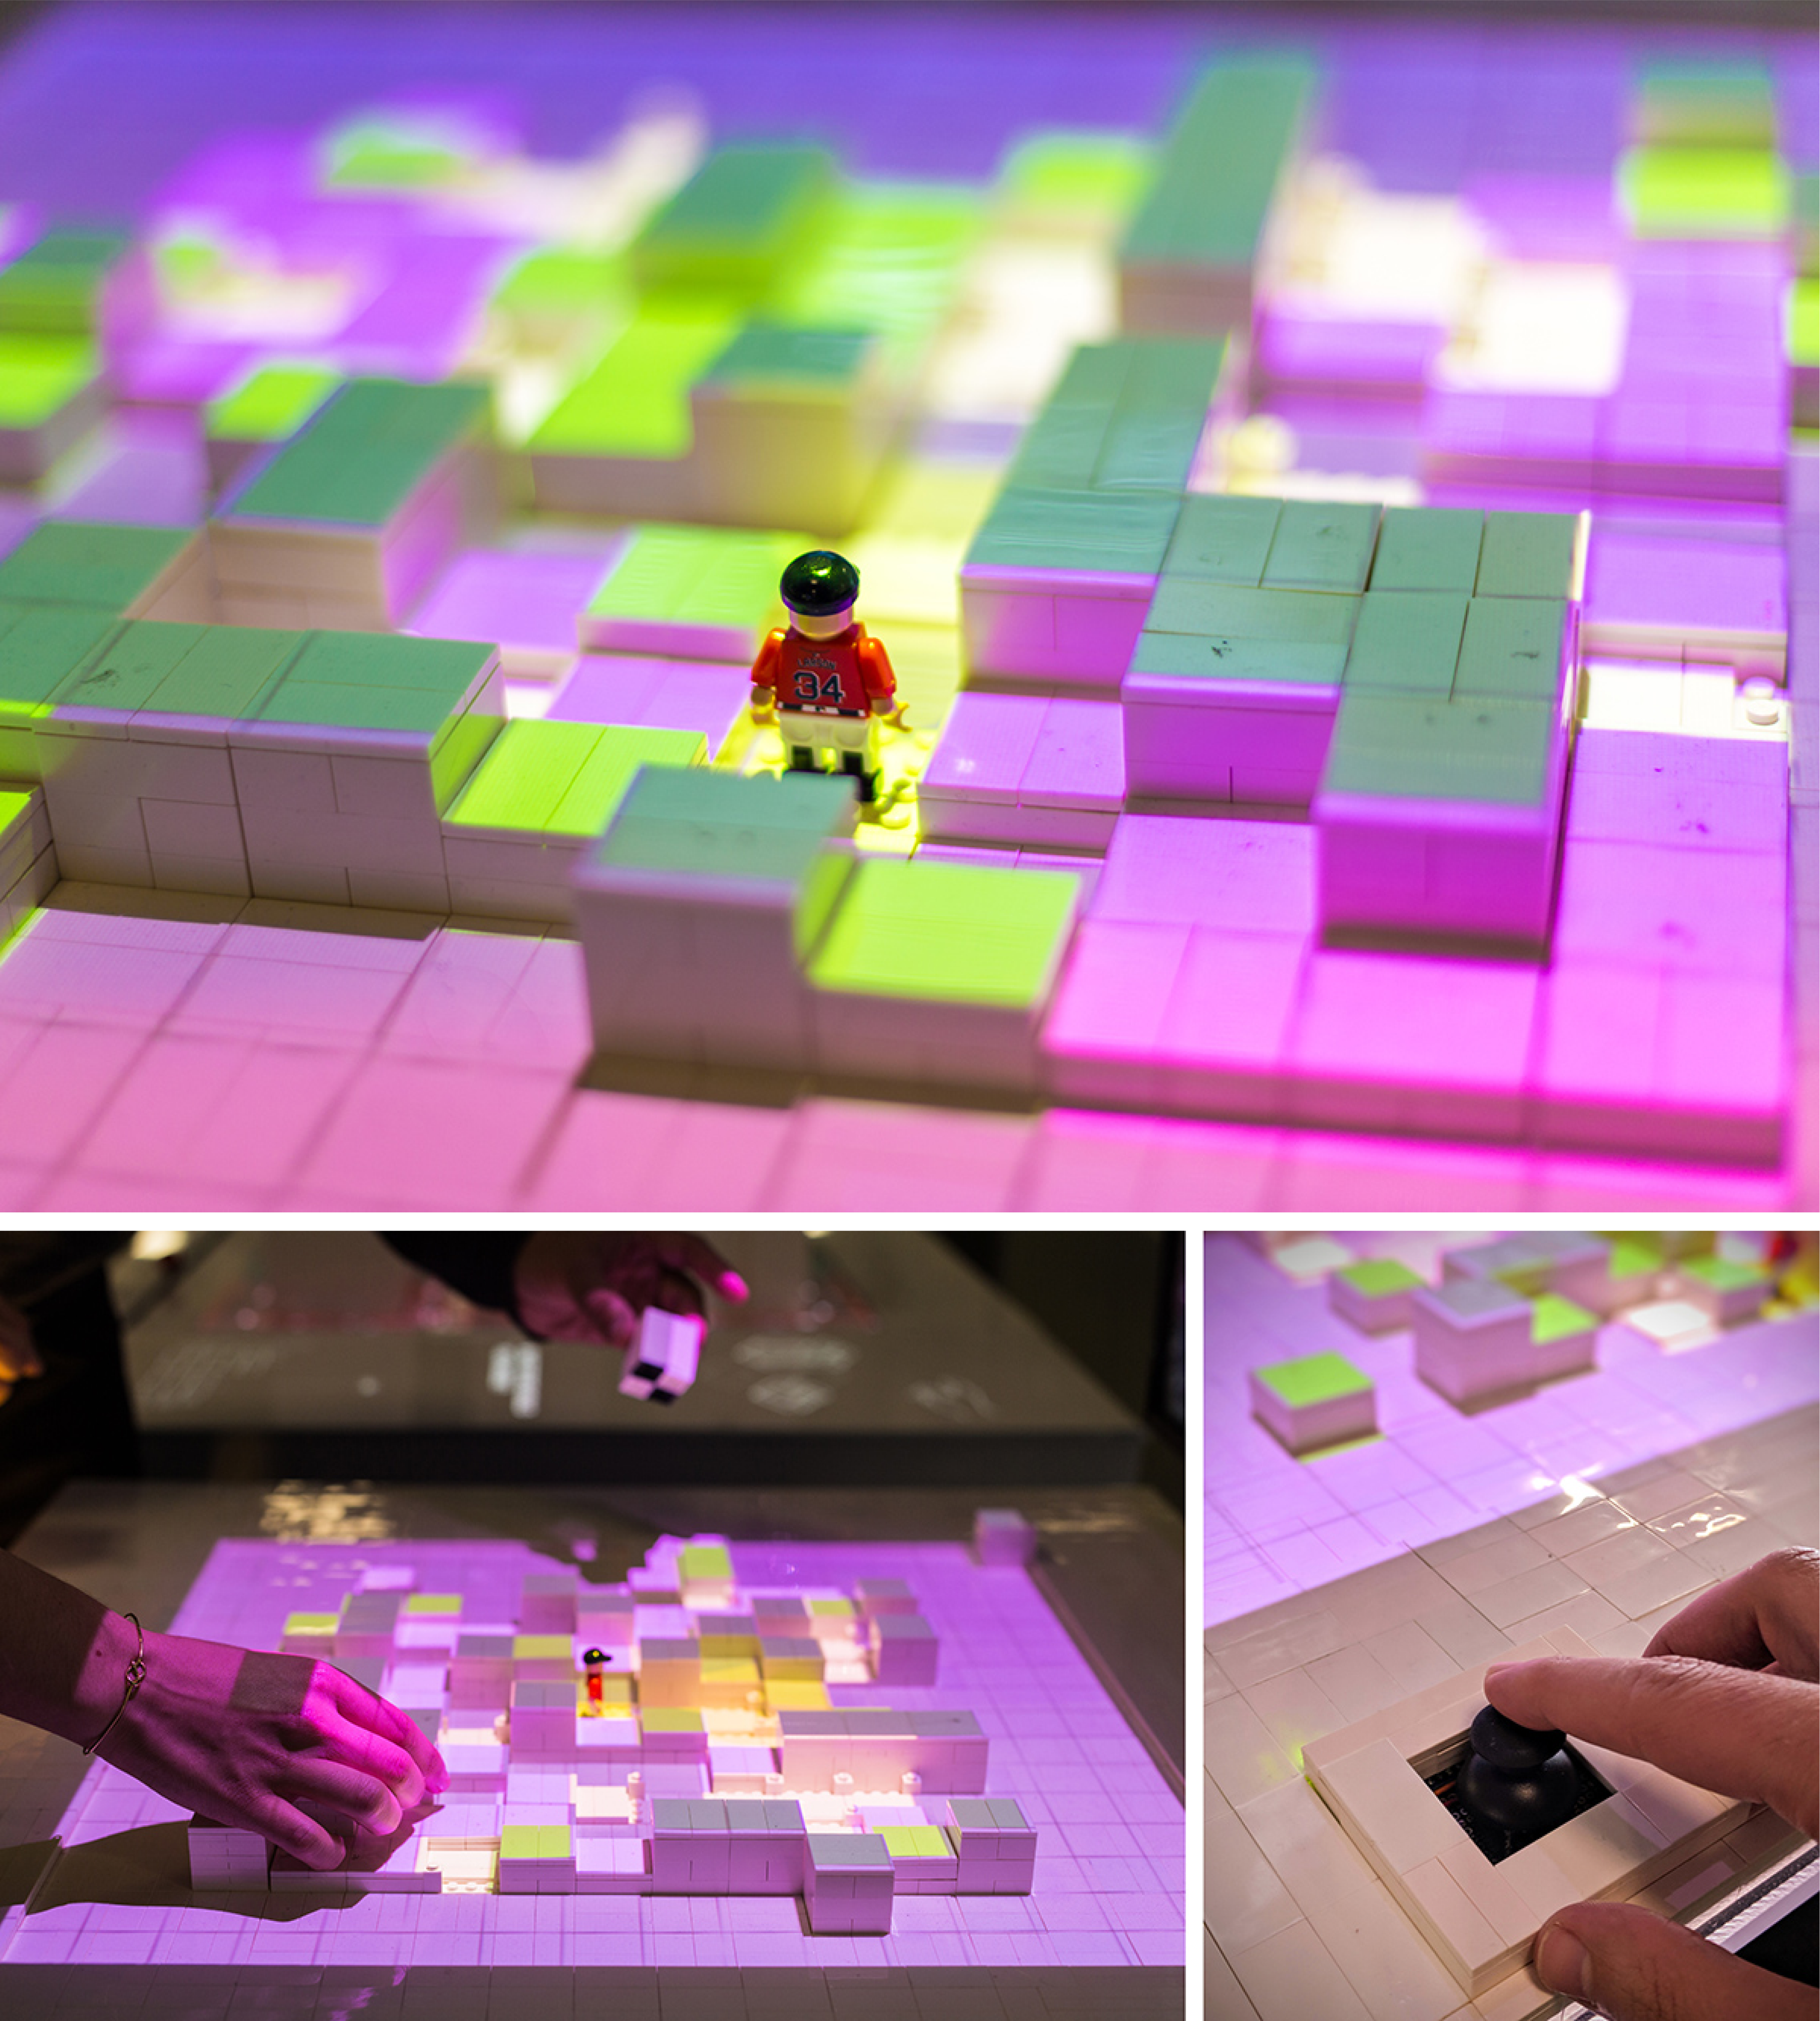
\includegraphics[width=0.7\columnwidth]{chapters/prediction/deepscope/figures/deepscope4.png}
            \caption{DeepScope TUI. (top) TUI and the Observer tile. (left) User interaction with grid-cells. (right) `Observer' viewing angle, depth and position is set via an Arduino game-pad}~\label{fig:deepscope_observer}
        \end{figure}


        \subsubsection{Observer}\label{observer}
        {
            The urban environment designed by the users is constantly captured by the `Observer' grid-cell. Similar to Lynch's `View form the Road' \cite{appleyard1964view}, this one-off unique CityScoPy pattern, mimics a virtual nomad traversing through the city. The Observer allows users to sets the position, point-of-view and angle of a virtual camera in the 3D scene, so that real-time visualizations will be predicted from that view. The Observer baseline parameters (such as FOV, Frustum and camera-height) were approximated to the camera calibration appendix of the Cityscapes dataset used in model training \cite{Cordts2016}. Additional camera controls were implemented to allow users to move, rotate, pan or zoom the Observer via custom game-pad joystick (see Figure \eqref{fig:deepscope_observer}).
        }

        \subsubsection{Tabletop Feedback}\label{deepscope-table-top}
        {
            As with other CityScope instances, DeepScope tabletop is used as both the design space and a canvas for data visualization. With each design iteration, an illuminated land-use diagram is projected onto the table-top, so that each tile is showing its respective pattern, name or parameters (density, land-use, etc.). The Observer position is displayed using perspective cone that indicates its current viewing angle and FOV (see Figure \eqref{fig:deepscope_dataflow}).
        }
    }

    %%%%%%%%%%%%%%%%% GAN  %%%%%%%%%%%%%%%%%% 


    \begin{figure}[!htb]
        \centering
        \includegraphics[width=0.5\columnwidth]{chapters/prediction/deepscope/figures/deepscope6.jpg}
        \caption{From site to prediction. This process depicts site selection, conversion to CityScope Schema, interaction, and prediction using the DCGAN model.}
        \label{fig:deepscope_pixelation}
    \end{figure}

    \subsection{Generative Model}\label{DeepScope-Generative-Model}

    {
        DeepScope uses a Deep Convolution Generative Adversarial Network (DCGAN) in order to generate street-view visualization in real-time. With each TUI interactions, the Observer viewpoint is captured as an input vector, used by the DCGAN model to predict an image (see Figure \eqref{fig:deepscope_dataflow}). The DCGAN generates an bitmap corresponding to the input vector, where each pixel in the input vector triggers the prediction of a corresponding pixel in the DCGAN output. The resulting image is then drawn onto the DeepScope feedback module.
    }

    \begin{figure}[!htb]
        \centering
        \includegraphics[width=1\textwidth]{chapters/prediction/deepscope/figures/deepscope0.jpg}\caption{(Top row) Model trained on Cityscapes dataset, deployed as node.js app. (Bottom row) TUI triggers DCGAN renderings.}~\label{fig:deepscope_arch}
    \end{figure}

    \subsubsection{Dataset and Model Training}\label{model-and-data}
    {
        Accurate pattern recognition using neural networks (NN) was already possible in the late 1980's \cite{lecun1989backpropagation}. However, generating new data that well concatenates a given dataset is still considered a complex problem in Machine Learning \cite{creswell2018generative}. Data generation using NN was greatly advanced with the introduction of Generative Adversarial Networks (GAN) \cite{Goodfellow2013}. GAN use two competing NN, a Generator and a Discriminator, that `adverse' one another; The Generator attempts to create new data (such as image, sound or text), and the Discriminator aims to nullify these data by comparing them to the distribution of a ground-truth data. The training is usually completed when the Generator can create close to indistinguishable samples which can fail the Discriminator \cite{pix2pix2016}.
    }


    \subsubsection{Image-to-Image Translation}\label{image-to-image-translation}

    {
        A variant of GAN is Conditional GAN (CGAN), in which both NN are given additional data that focuses the generation on specific targets \cite{mirza2014conditional, salimans2016improved}. A notable use-case of CGAN is a pixel-wise conditional generation of images, known as Image to Image Translation or `pix2pix' \cite{isola2017image, pix2pix2016}. In pix2pix, pairs of images are used for training, where the pixel values of one image are used as labels (also known as `classes') of the other. This allows pixel-level prediction using spatial classification of regions in the image \cite{arjovsky2017wasserstein, zhu2017unpaired}. In practice, CGAN extends the classic GAN zero-sum objective function with additional class data so that:
        \begin{equation} \label{deepscope-gan-objective-function}
            \min_G \max_D V(D, G) = \mathbb{E}_{\bm{x} \sim p_{\text{data}}(\bm{x})}[\log D(\bm{x} | \bm{y})] + \mathbb{E}_{\bm{z} \sim p_z(\bm{z})}[\log (1 - D(G(\bm{z} | \bm{y})))]
        \end{equation}
        where function ${V}$ of the Generator and the Discriminator ${G, D}$ attempts to minimize a delta between ground-truth data ${x}$ (in this case, the pixel data) and ${z}$, which is the accumulated pixel distribution learnt on each training step (see Figure \eqref{fig:deepscope_epoch}). Unlike classic GAN, $\log_{D(\bm{x} | \bm{y})}$ denotes that the additional `class' data ${y}$ conditions the learning on both data \textit{x} as well as on ${y}$ class. In this respect, CGAN generator do not only generate data with resemblance to the learnt distributions, but can closely mimic details in the data structure. DeepScope implements a variant of pix2pix that is fast and lightweight enough for real-time predictions in web browsers of low-tier devices.
    }


    \subsubsection{Cityscapes Dataset}\label{cityscapes-dataset}
    {
        The DeepScope DCGAN model was trained on the Cityscapes dataset \cite{Cordts2016}. Cityscapes is composed of pairs of street-view images taken using a dashcam around 50 European cities, during different seasons, daytime and weather conditions. Each pair includes a street-view image and a corresponding segmented image with 30 semantic labels (`classes'). These labels represent different streetscape classes, from buildings and roads to license-plates and road signs. For DeepScope, a pre-processing algorithm was designed to remove motion-blur, increase sharpness, saturation and remove color-casting, which were common in a shots taken by a moving vehicle. This pre-processing tools was built in Python OpenCV \cite{opencv_library}.

    }

    \subsubsection{Model Architecture and Performance}\label{dCgan-model-architecture-and-performance}
    {
        The model architecture of DeepScope was designed to allow fast predictions and portability for web-based devices. The Generator network has 16 layers with a U-Net encoder-decoder structure \cite{ronneberger2015u}. For performance purposes, the Discriminator has only 5 layers and is using Leaky ReLU activation that has been shown to improve stability in training \cite{Radford2015}. Commonly, DCGAN models benefit from higher number of filters \cite{ronneberger2015u}, however more filters also increase the model size, which can impact real-time performance and usability in low-tier devices. In order to still maintain attention to fine details, a shallow network design with a random up-sampling of 150\% was used \cite{isola2017image}. This network allows deployment on client-side browsers or mobile devices where TensorFlowJS is supported \cite{smilkov2019tensorflow}.
    }



    \begin{figure}[!htb]
        \centering
        \includegraphics[width=0.3\columnwidth]{chapters/prediction/deepscope/figures/deepscope1.jpg}
        \caption{Test samples during training. Right column shows quality degradation beyond $\sim$200 epochs.}~\label{fig:deepscope_epoch}
    \end{figure}


    \subsubsection{DCGAN Training and Results}\label{dCgan-training-and-results}
    {
        20 training sessions were conducted with 16, 32, 64 and 128 filters, and 50 to 2000 epochs. Resulting models were converted to a \verb|JSON| format and tested for stability and response time on various browsers. A trained model with 64 filters and 200 epochs showed the best overall results. Models with less filters produced low-quality results; models with up to 2000 epochs demonstrated inconsistencies and `mode collapse' \cite{arjovsky2017wasserstein}.
    }


    \subsubsection{UI Performance Test}\label{deepscope-platform-and-user-interaction}
    {
        In order to avoid interaction latency, two asynchronous processes were used: (i) prediction process, and (ii) TUI interaction response. In user tests, the DCGAN model predicted at $0.66 sec/prediction$ on an average desktop system used by CityScope instances; the TUI has a fixed response interval of 50ms. Although DCGAN predictions slightly trails the TUI, the observation showed that users tend to focus their attention to the horizontal TUI before expecting the DCGAN output. Therefore, the overall user experience could be considered real-time with continuous design-and-feedback loops \cite{deber2015much}.
    }


    \subsection{Discussion}\label{deepscope-discussion}
    {
        DeepScope is a CityScope module which uses a real-time neural-network model to provide early stage urban-design visualization of skylines and streetscapes. Different from previously explored analysis modules, DeepScope aim is not to predict the impacts of urban intervention with respect to physical urban systems; Instead, DeepScope is meant to offer an implicit impression of the prospective development during the design process. Alongside mobility, energy, and other spatial-physical metrics, DeepScope can be used to `hallucinate' the impact of urban interventions, thus adding another way to evaluate urban transformation. The rest of this section discusses the strengths, weaknesses, threats and opportunities of this work.



        \subsubsection{Strengths}\label{strengths}
        {
            Early urban-design stages have major impacts on the spatial organization of cities, but commonly lack sufficient design representation and clear `image' \cite{Batty2000}. DeepScope is designed to allow experts and non-professionals alike to collaboratively experiment with urban-design scenarios and real-time feedback. The platform can augment early stages of urban-design with near real-life street-view visuals. The `unpolished' nature of the visualizations forces designers and regulators to focus on the overall `Image of the City', instead of highly-specific design details \cite{lynch1960image}. Unlike traditional tools, the complexity of creating a detailed urban scene is carried out by a lightweight, pre-trained neural network, which is triggered by an intuitive TUI.
        }

        \subsubsection{Weaknesses}\label{weaknesses}
        {
            Despite their promise, GAN have several drawbacks. First, they require large and properly labeled datasets. For example, creating a Cityscapes-like dataset for other geographies will involve significant efforts. Several emerging methods suggest decoupled \cite{zhu2017unpaired} and label-less learning \cite{lucic2019high}, which can simplify the labeling effort. Nevertheless, dataset collection and partial labeling would still be required. Moreover, GAN tend to be inconsistent during learning process, as explored in Subsection \nameref{dCgan-training-and-results} \cite{shin2017continual}. Lastly, the DeepScope GAN would not be able to visualize non-street view angles: Since the Cityscapes dataset was captured using a vehicle dashcam, only matching angles produce reasonable predictions \cite{salimans2016improved}. This issue is common in other supervised networks, and requires either non-supervised methods or more extensive datasets.
        }


        \subsubsection{Threats}\label{threats}
        {
            The rising popularity of GAN is attributed to their ability to `create'; Nevertheless, GAN tend to produce unpredictable results. When it comes to the design practice, certain degree of `creative freedom' might be desired, yet unpredicted tools might cause resentment or misleading impressions. For example, in DeepScope, the same street-view angle with the same urban-design setup can produce different visual results if ran twice. Additionally, NN are strictly bounded to their architecture and training data. Tempered network or adversarial datasets can greatly affect the outcomes of the model and inject bias into the results. With machine-learning tools becoming mainstream in the design industry, these concerns should be addressed by testing, validating and open-sourcing design tools, models and data.
        }


        \subsubsection{Opportunities}\label{opportunities}
        {
            DeepScope can be improved in several aspects: First, emerging network architectures and training parameters can improve the DCGAN results. Other methods, such as VAE or auto-GAN, can produce finer results with greater control \cite{mescheder2017adversarial}. As well, extending the training datasets to different urban environments could yield more versatile representations and geographical relevancy. Lastly, the TUI can be improved to include multi-scale environments and more finer-grained editing capability.
            \newline
            More broadly, DeepScope might hint to a future of insightful urban-design tools, spanning beyond digital rulers and drafting aids. Such tools would not only expedite tedious tasks, but might be able to leverage the power of advanced computation and become digital design `companions'.
        }
    }
}
